\documentclass[a4paper,onecolumn,11pt]{article}
%%%%
\renewcommand{\familydefault}{\sfdefault}%
%%%

%Packages%%%%%%%%%%%%%%%%%%%%
\usepackage[margin=2cm]{geometry} %this assures 2cm margin on all sides
\usepackage{graphicx}% to include figures
\usepackage{array}%
\usepackage{hyperref}
\usepackage{listings}
\hypersetup{linkcolor=blue, pdftitle={Quantifying Software Quality through Data Change Validation}, pdfauthor={Dominic Roberts}, pdfsubject={Research Proposal Assignment -- January 2018}, pdfkeywords={software quality, software testing, mutation testing, genetic algorithms} }
%%%%%%%%%%%%%%%%%%%%%%%%%%%%%%%%%%%%%%%%%%%%%%%%%%%%%%%%%%%%%%%%%%%%%%%%%%%%%%%%%%%%%%%%%%%%%%%%%%%%%%%%%%%%%%%%%%%%%%%%%%%%%%%%%%%%%%%%%%%%%%%%%%%%%%%%%%%%%%%%%%%%%%%%%%
%%DOUBLE QUOTE and SINGLE QUOTE Commands%
\newcommand{\qq}[1]{\textquotedblleft#1\textquotedblright}%
\newcommand{\q}[1]{\textquoteleft#1\textquoteright}%
\pagenumbering{arabic}%
%\setcounter{page}{-1}%
\begin{document}
\title{\vspace{-2.5cm}Solving the NQueens problem with Genetic Algorithms seeded by lower dimension results}
\author{\textbf{Dominic Roberts}\\
\textbf{P17201056}\\
MSc Intelligent Systems, De Montfort University
}%
%%%%%%%%%%%%%%%%%%%%%%%%%%%%%%%%%%%%%%%%%%%%%%%%%%%%%%%%%%%%%%%%%%%%%%%%%%%%%%%%%%%%%%%%%%%%%%%%%%%%%%%%%%%%%%%%%%%%%%%%%%%%%%%%%%%%%%%%%%%%%%%%%%%%%%%%%%%%%%%%%%%%%%%%%%
% make the title area
\maketitle
\thispagestyle{empty}
%%%%%%%%%%%%%%%%%%%%%%%%%%%%%%%%%%%%%%%%%%%%%%%%%%%%%%%%%%%%%%%%%%%%%%%%%%%%%%%%%%%%%%%%%%%%%%%%%%%%%%%%%%%%%%%%%%%%%%%%%%%%%%%%%%%%%%%%%%%%%%%%%%%%%%%%%%%%%%%%%%%%%%%%%%

\section{Abstract}
The 8-Queens problem was devised by Max Bezzel in 1848 and consists of a challenge to place 8 Queens on a chess board such that none of the Queens are able to attack another Queen. The more general form of the problem is known as the N-Queens problem where N denotes the dimensions of the board and subsequent count of Queens. The problem is known to be NP-Complete \cite{Complexity}. There have been many different solutions found for the problem, the original solution was provided by Franz Nauck in 1850. It has been used as a benchmark for AI research due in part to it being an Np-Complete problem that is easy to explain to anyone with a basic understanding of Chess. Due to its popularity there have been numerous attempts to resolve the problems using Genetic Algorithms (GA) previously. However, this paper describes a technique that uses the outcomes from lower dimensional evaluations to seed the GA in order to massively improve the performance in searching for solutions in the given dimensions. By reusing previous successful solutions from a lower n-dimensionality it aims to show that there is a close correlation between the results from each dimension and that combinatorial problems like the N-Queens problem can be simplified by applying lower dimensional solutions to higher order problems.

\section{Introduction}
In the game of Chess the Queen is the only piece on the board that is permitted to move any number of spaces horizontally, vertically and diagonally. On a standard 8x8 board it can attack up to 21 different squares in a single move. In 1848 Max Bezzel proposed a puzzle for calculating a configuration whereby 8 Queens can be placed on a board without any two pieces being able to attach each other. This problem, known as the 8-Queens problem, has a more generic variant that imposes the same rules on boards of any topology such that the for N dimensions, there are NxN squares on the board and N Queens to be placed. Since the initial proposition of the puzzle there have been many different approaches to solving it. The first person to successfully find all 92 placements of the original 8x8 board was Pauls \cite{Pauls} in 1874. Work has continued since to resolve the solutions for higher dimensions, currently the maximum dimensions for which all solutions have been proven is 27, for which there are 234,907,967,154,122,528 solutions a result that took over a year of computing time to calculate\cite{27Queens}. This limitation is due to the enormous number of solutions at higher dimensionalitys. The possible combinations of a board layout is $N^{N}$ and so the possible valid permutations grows exponentially as the dimensions are increased. Table 1. lists a selection the number of permutations for the board layout.

\begin{table*}[!htbp]
	\begin{tabular}{|l |l|} 
		\hline\
		Dimensions & Combinations \\
		\hline\
		8 & 16,777,216 \\ 
		9 & 387,420,489 \\
		10 & 10,000,000,000 \\
		15 & 437,893,890,380,859,375 \\
		20 & 104,857,600,000,000,000,000,000,000\\
	\hline
	\end{tabular}
	\caption{Possible Permutation for Queen positions on a N Dimensional Chess board} 
\end{table*}

The first implementation of a Genetic Algorithm (GA) to solve the problem was by Crawford \cite{Crawford} in 1994. Since this point a variety of Heuristic algorithms have been configured to resolve the problem \cite{AdvanceMutation} \cite{ACO} \cite{comparison} \cite{PSO}. Although the N-Queens puzzle is NP-Hard it is a very simple to describe to anyone familiar with the game of Chess. This has led to it becoming a benchmark problem for the development and testing of Heuristic solutions. Brute force approaches to solving the problem are effective at calculating the results for all combinations over the lower ranges of dimensions, but as the number of possible combinations increases, so the time required to evaluate all potential options becomes prohibitive.

This paper introduces a variation on the standard Genetic Algorithm. The technique developed seeds the initial search locations for the algorithm with result sets obtained from a lower dimension. Valid board configurations from a smaller board are enhanced with additional fields to boost the dimensions to the required size and then set as the initial genome location in new clusters of genomes. The rest of this paper is organised as follows the next section will give more detail of the N-Queens problem, this is followed by an overview of Genetic Algorithms and their implementations. An analysis of related works is then given to give additional context to the problem and existing research into the use of Heuristic algorithms to solve it. The subsequent section will detail the approach that has been developed in this paper and that is then followed by an analysis of the results obtained. Finally, the paper will discuss the outcomes and conclusions from the research and indicate a number of potential areas for further investigation.

\section{N Queens}
The N-Queens problems requires N Queens to be placed on an $NxN$ chess board such that no two Queens are able to attack each other. On an N dimensional board there are $N^{N}$ possible placements for the N Queens. However, as any Queen placed on the same column or row as another would immediately invalidate that combination. Thus the permutations can be reduced to !N configuration as each piece is restricted to a single piece per column and per row.

\begin{figure}[!htbp]
	\centering	
	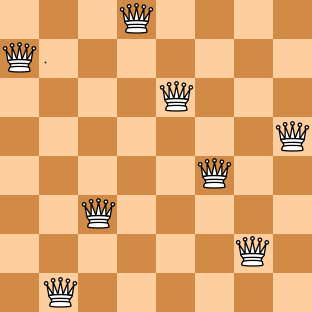
\includegraphics[width=6cm, height=6cm]{Valid8QueensSolution}
	\caption{An example of a valid 8 Queens solution where no 2 Queen placements are able to attack another Queen.}
\end{figure}

It is possible to determine valid results for all dimensions above 3. There are no possible solutions for N=2 or N=3. The following table gives the number of available solutions for a range of values for N. As the number of dimensions increases the possible solutions also increases for all values apart from 6 for which there are only 4 valid configurations. 

\begin{table*}[ht]
\begin{tabular}{|p{2cm}|p{6cm}|p{6cm}|} 
		\hline\
		Dimensions & Solutions & Unique Solutions \\
		\hline\
		4 & 2 & 1 \\ 
		5 & 10 & 2 \\
		6 & 4 & 1 \\
		7 & 40 & 6 \\
		8 & 92 & 12 \\
		9 & 352 & 46 \\
		10 & 724 & 92 \\
		15 & 2,279,184 & 285,053 \\
		20 & 39,029,188,884 & 4,878,666,808 \\
		25 & 2,207,893,435,808,350  & 275,986,683,743,434 \\
		26 & 22,317,699,616,364,000 & 2,789,712,466,510,280 \\
		\hline
	\end{tabular}
	\caption{The number of Solutions and Unique Solutions for a range of values for N}
\end{table*}

Table 2 gives the number of solutions along with the unique variants at each dimension. For every solution to the problem it is possible that there is also a rotational or reflected variant that could also be a valid configuration. By rotating the board through 90, 180 and 270 degrees or reflecting along the central X and Y axis of the board then further valid solutions can be found.

\begin{figure}[!htbp]
	\centering	
	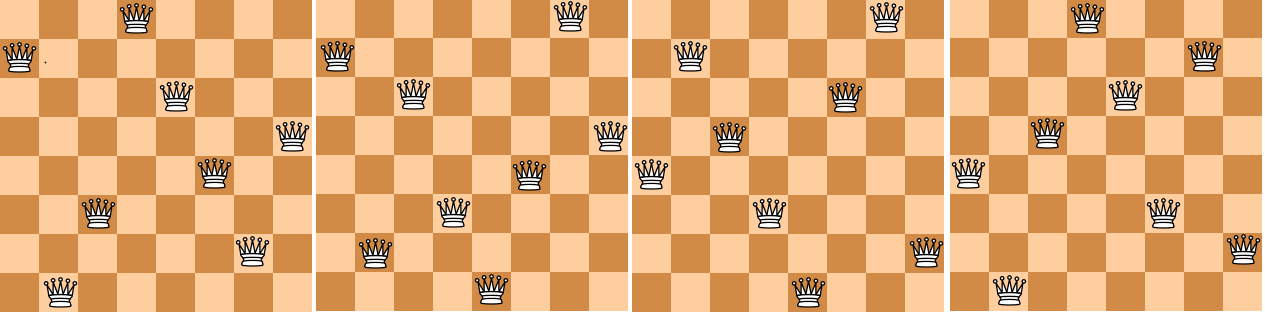
\includegraphics[width=16cm, height=4cm]{NQueensRotations}
	\caption{By rotating a configuration through 360 degrees further valid solutions can be derived.}
\end{figure}

\begin{figure}[!htbp]
	\centering	
	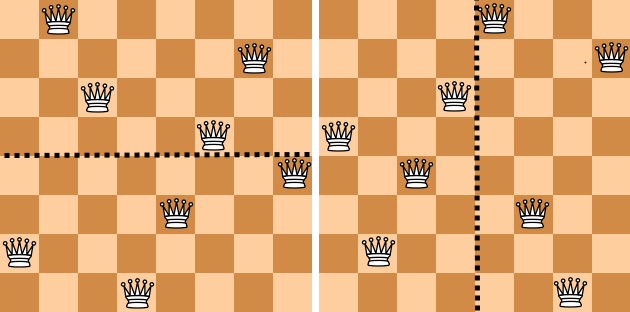
\includegraphics[width=8cm, height=4cm]{Valid8QueensReflected}
	\caption{By reflecting the layout along the X and Y axis other valid solutions can be derived.}
\end{figure}

The ability to locate potentially an additional 5 solutions from an initial configuration improves the performance of a Search algorithm. Each time a new solution is found analysing each of the transformations can yield multiple valid layouts.

\subsection{Related Works}


\subsection{Applications}

Although it is generally considered to be merely a mathematical puzzle there are numerous real world applications for solutions to the problem. Research in to the puzzle has been used to detect database deadlocks \cite{Deadlock}. The search algorithm was re-purposed to find locking designs where no two locks could affect each other. Further applications have been found by Tanik \cite{SIMD} \cite{Circulant} for conflict free, fast, parallel array access in software. When there are asynchronous attempts to read and write to the same array structures in software locking of memory is generally required, this reduces the efficiency of memory access. The research by Tanik applied the principles from an N-Queens solution to ensure horizontal, vertical and diagonal access to the storage structures would be lock free.

There have been numerous areas of image processing that have also drawn influence from N-Queens to propose solutions to issues in motion detection \cite{WSN}. In the work by Stojkoska et al. they use the placements of Queens on an NxN board to reduce the number of pixels on an image that need to be tested to detect the motion of objects between two images. The research shows that they can successfully reduce the pixels to be tested from $N^2$ to just Nx2. A single configuration of Queens showed 75\% accuracy, whilst overlaying with a solution reflected in the Y-Axis increased performance to 95\%.

\section{Implementation}
\subsection{Genetic Algorithm}
It can be seen from Figure 1 that where there are no two pieces are on the same Horizontal or Vertical then the only concern when resolving the problem is along the diagonals. Representation of the board can be reduced to a tuple of integer values such that a valid solution for 8-Queens can be represented as (1,7,5,0,2,4,6,5) where 0-based indexing has been used. The storage structure for genome members can thus be an array of integer values. The array index infers the column and the value represents a row on that column.

The implemented evaluation function receives an N length array of integers and returns the number of attacking conflicts present on the board layout described. A result of 0 conflicting positions indicates that a valid solution has been located. Using the array representation calculating the conflicts is a simple two step process. Step 1 is to detect duplicate values within the input array, each duplicate is counted as a conflict. Step 2 is to locate opposing diagonals, given two board locations c1 and c2 which are represented by the structure (x,y) where x is the column index and y is the cell value. Diagonals can be determined by: 
\begin{lstlisting}
 if abs(currentX - boardX) == abs(currentY - boardY):
	attackingQueens += 1
\end{lstlisting}

The generation of genome sequences and their subsequent mutations is required to ensure that no duplicate values are entered in to the array. The addition of duplicate values will immediately indicate an invalid solution. To ensure this, the process for updating a genome pattern was altered so that the transformations occur through the alteration of two positions within the current sequence and not through the introduction of new values in to the current values. New sequences are generated through a stochastic mutation process where two nodes are selected from the genome and their positions are swapped. No attempt is made to cross over parts of the sequence between differing members as this will lead to duplicate items in the structure. Duplication should be avoided in the genome generation as it is an automatic failure of the N-Queens problem. To ensure that no duplicates appear in the genome, switching of segments between two instances i.e. cross-over and randomly selecting a replacement value for an existing node i.e. standard mutation, are both avoided. Instead two locations in the sequence are selected at random and the values at those locations are switched. The tests performed on the solution showed a dramatic improvement in performance when the algorithm was exercised with variants of this transformation.

\begin{figure}[!htbp]
	\centering	
	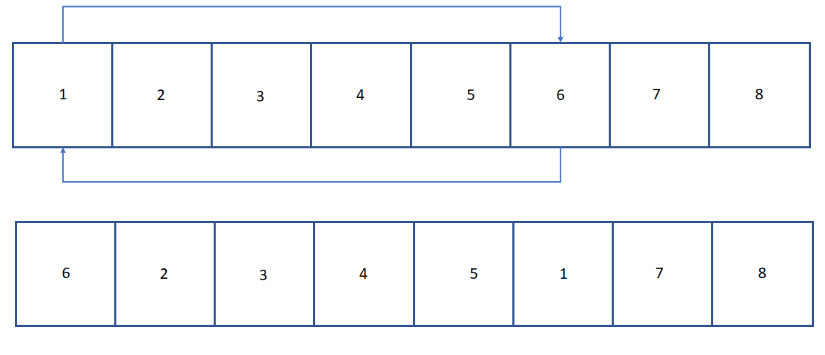
\includegraphics[width=10cm, height=6cm]{SimpleCrossOver}
	\caption{By only exchanging the locations of items within the same set duplicates can be guaranteed not to occur.}
\end{figure}

As an unconstrained problem, an N dimensional board would have $N^N$ possible placements to consider. By enforcing the single value per column and removing the possibility for duplicates the problem space has been reduced to a combinatorial problem with a size of $!N$. This is a significant reduction in size. For a standard 8 X 8 board this reduces the search space from 16,77,216 to 40,320.

The implemented genetic algorithm starts by generating clusters of genomes known as Demes \cite{Demes}. The Demes group genomes together around an initial starting location and on each iteration are modified in relation to the best performing Deme member. The use of these clusters allows multiple sections of the search space to be investigated simultaneously. The size of each group is initiated from a starting parameter set that can be configured per run of the algorithm. Each genome in the Deme is instantiated with a starting location which is a single transformation away from the parent value. 

When the members of each Deme is generated they are assigned to a mini tournament of 3 members taken randomly from the Deme. On each iteration the members each calculate their current fitness value via the N-Queens evaluation function. Each of the mini-tournaments within a Deme are then contested, the competitor with the best fitness, over the duration of the members lifetime and not just a single round, is retained for the next iteration. All losing members of the tournament are discarded. New Deme members are then produced as offspring of the winners and a new tournament is created consisting of the parent and it's two new offspring. Through this process the population maintains the best performing locations in to the next iteration and the weaker members are discarded.

On each iteration of the process the Demes are aged, if no improvement has been made to the performance of the winning members then the age is incremented, when improvement is made then the age counter is reset to 0. The process has a fixed maximum age per Deme and once a group matures beyond this threshold it is removed from the group and replaced by a new Deme that is seeded to start at a new location.

The initial location for each Deme and subsequently the root location for all of its members is taken from the list of valid results that have been located for runs on a lower dimension. For example, executing a run with a value for N = 8 will import the result data extracted during a run with N = 7. The new, unknown node value is then set to the value not used in the lower dimensions. A repository of the input values is imported during the initialisation phase of the algorithm and referenced each time a new location is required. The imported data is accessed iteratively rather than stochastically to ensure that each dataset is evenly distributed. A count is held for each usage of a single sequence, this is then used to alternate the root index position in the target location i.e. for a 7 node sequence it alternates between starting at offset 0 and 1 in the target sequence.

\begin{figure}[!htbp]
	\centering	
	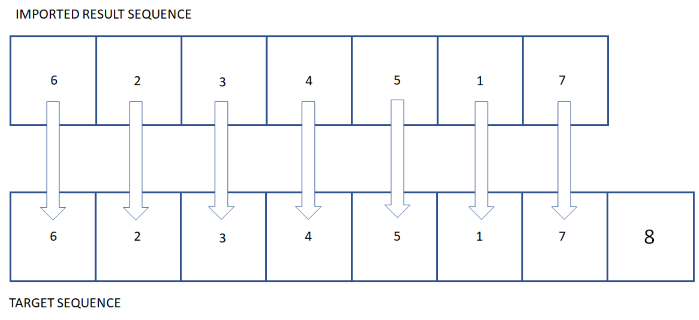
\includegraphics[width=10cm, height=6cm]{ImportSequence}
	\caption{The imported result set from a 7X7 board is used to initiate the search for an 8X8 board.}
\end{figure}

\section{Results}
The algorithm described in the previous section is a stochastic process that will not achieve consistent results on each execution, for this reason it was run 10 times per board size to gauge an average performance. An alternative approach was also used to benchmark the efficiency of seeding the starting point against a standard unseeded implementation. The unseeded alternative selected a starting location through a random process that ensured there were no duplicated values in the sequence. This was achieved by filling an array with each of the possible values, then selecting a position in the array at random and placing the value at that index in to the sequence. The extracted value was then removed from the array and it's length shortened accordingly.

The algorithms were then compared for two properties, the number of evaluations required to locate all known valid sequences in an N-Dimensional board and the number of evaluations required to locate a first valid solution. The seeded solutions used the results of N-1 dimensions to provide the seed locations.

\begin{table*}[ht]
	\begin{tabular}{|p{2cm}|p{6cm}|p{6cm}|} 
		\hline\
		Dimensions & Seeded Solution & Unseeded Solution \\
		\hline\
		8 & 14,935 & 18,740 \\
		9 & 338,889 & 191,231 \\
		10 & 1,450,501 & 865,135 \\
		11 & 11,395,148 & 7,447,889 \\
		\hline
	\end{tabular}
\caption{The average number of evaluations required for each algorithm to find all solutions and differing dimensions.}
\end{table*}

The statistics in Table 3 indicate that the number of evaluations required for the seeded solution to locate all valid combinations performed increasingly poorly against the unseeded variant. At the lower dimensions seeding was an optimal solution but as the N increases the performance deteriorates comparatively. It is possible this is due to the exponential growth in the number of valid solutions on increments to N. 

\begin{figure}[!htbp]
	\centering	
	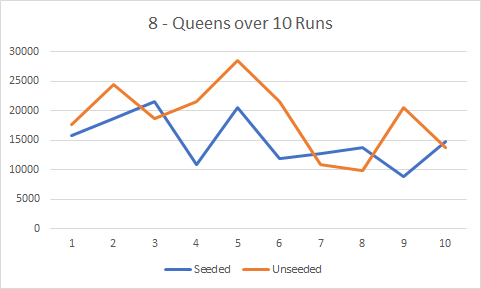
\includegraphics[width=10cm, height=5cm]{8QueensAllValues}
	\caption{Comparison of the number of evaluations required to obtain all results for N=8.}
\end{figure}

\begin{figure}[!htbp]
	\centering	
	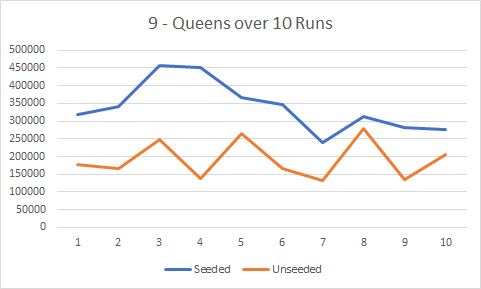
\includegraphics[width=10cm, height=5cm]{9QueensAllValues}
		\caption{Comparison of the number of evaluations required to obtain all results for N=9.}
\end{figure}

\begin{figure}[!htbp]
	\centering	
	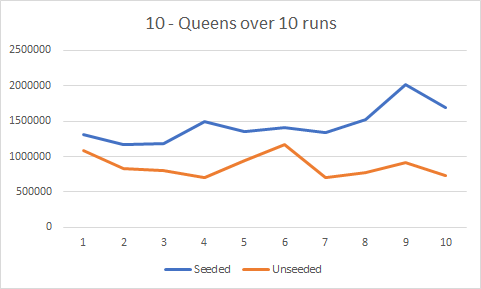
\includegraphics[width=10cm, height=5cm]{10QueensAllValues}
		\caption{Comparison of the number of evaluations required to obtain all results for N=10.}
\end{figure}

\begin{figure}[!htbp]
	\centering	
	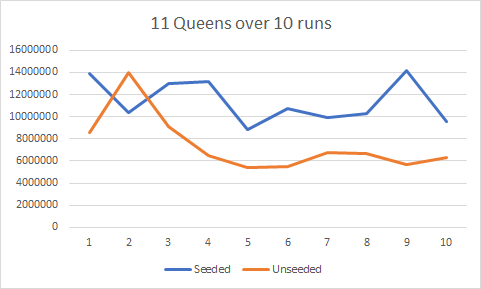
\includegraphics[width=10cm, height=5cm]{11QueensAllValues}
		\caption{Comparison of the number of evaluations required to obtain all results for N=11.}
\end{figure}

Although the evaluation of an N=8 board is marginally faster on average when seeded there is a distinct advantage overall for unseeded locations. During the test execution it was noticed that there is a distinct increase in performance for locating the first solution from the seeded implementation. In the work by Khan et al. \cite{ACO} evaluations of the performance was against the time taken to find the first valid solution rather than locating all solutions. As the number of dimensions increases it becomes of increasing relevance to locate a single valid solution.

Studying the performance of the seeded algorithm it appeared that during the latter stages of the process that performance distinctly drops off.  It would appear that initialisation with previous result sets helps the algorithm to rapidly locate a new valid solution based off those of lower dimensionality. As the solutions close to those seeded locations are uncovered the remaining valid sequences are further away from the starting location in terms of mutations required. This causes the algorithm to become less performant than when purely random sequences are used as starting positions for the collection of Demes.

\begin{table*}[ht]
	\begin{tabular}{|p{2cm}|p{6cm}|p{6cm}|} 
		\hline\
		Dimensions & Seeded Solution & Unseeded Solution \\
		\hline\
		21 & 525.6 & 180,080 \\
		22 & 227.5 & 211,205 \\
		23 & 263.4 & 294,635 \\
		24 & 623.3 & 257,045 \\
		25 & 525 & 386,255 \\
		26 & 938.7 & 389,225 \\
		27 & 1,009.5 & 511,115 \\
		28 & 338.9 & 612,505 \\
		29 & 1,152.4 & 697,310 \\		
		\hline
	\end{tabular}
	\caption{The average number of evaluations required for each algorithm to find a first solution and differing dimensions.}
\end{table*}

The results in Table 4 show the average number of evaluations required to find a first valid solution for values of N from 21 to 29. The table compares performance between seeded and unseeded variants of the Genetic Algorithm. It is very clear to see from this that the use of a starting location that is valid for a lower dimension dramatically reduces the computation required. The average number of evaluations holds steady as N increases whereas for randomly selected locations there is an increasing complexity in locating a first solution.

\begin{figure}[!htbp]
	\centering	
	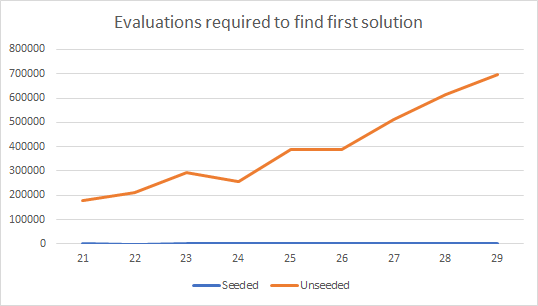
\includegraphics[width=10cm, height=5cm]{EvaluationsFirstSolution}
	\caption{Comparison of the required evaluations to obtain a first valid sequence for N=21 - 29.}
\end{figure}

The clear increase in performance for the location of a first solution is in contrast to the performance in selecting all locations. The experiments showed that for each value of N greater than 8 the stochastically selected starting locations out performed that of the seeded algorithm. On closer inspection of the results it is apparent that this is caused by a poor performance at the identification of the final available results. The variant of the algorithm using predetermined sets of results becomes stuck in its local minimum and requires greater computation time to locate solutions that are unseen in lower dimensions.

\begin{figure}[!htbp]
	\centering	
	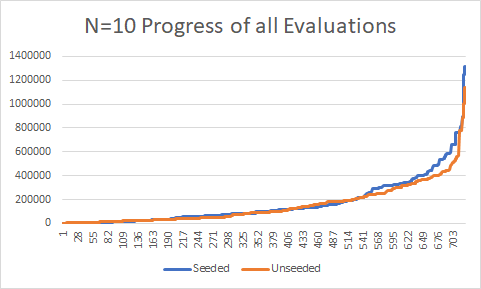
\includegraphics[width=10cm, height=5cm]{N10AllEvaluations}
	\caption{Comparison of the progress of solution identification for N = 10.}
\end{figure}

\begin{figure}[!htbp]
	\centering	
	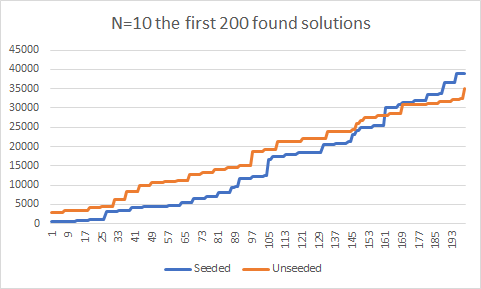
\includegraphics[width=10cm, height=5cm]{First200Progress}
	\caption{A closer inspection of the initial progress made in locating solutions for N = 10.}
\end{figure}

Figures 11 and 12 indicate that using the known locations as starting points for the Demes gives an advantage over randomly selected locations during the initial phases but is surpassed when locating the tail end of solutions. 

Results for each dimension are based up on the values obtained at a lower dimension though tests show that only a small number of source values are required to achieve a valid solution at the higher N. To obtain a sequence at N = 100 sequences are required for N = 99. Tests were performed to gauge how many evaluations were required to find a resolution for N = 100 by initiating the tests with only a set of solutions for N = 7. The test run was executed by incrementing the step 1 dimension at a time from N= 8 to N = 100, on each iteration the results are stored in memory and passed to the process on commencement of each step. The intention is to evaluate how long it would take to obtain a solution for N = 100 having started with a basic level of seed information. The result of tests showed that it was possible to obtain a first valid solution in only 240,899 evaluations.

\begin{figure}[!htbp]
	\centering	
	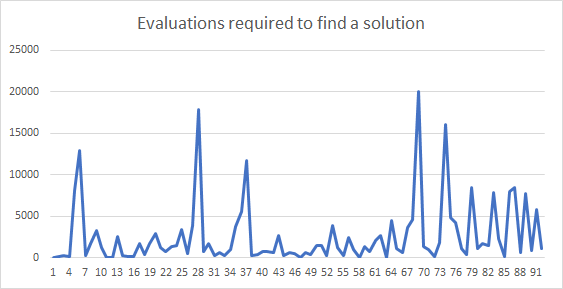
\includegraphics[width=10cm, height=5cm]{EvaluationsPerDimension}
	\caption{This figure shows the number of evaluations required to locate a first solution at each dimension.}
\end{figure}

\begin{figure}[!htbp]
	\centering	
	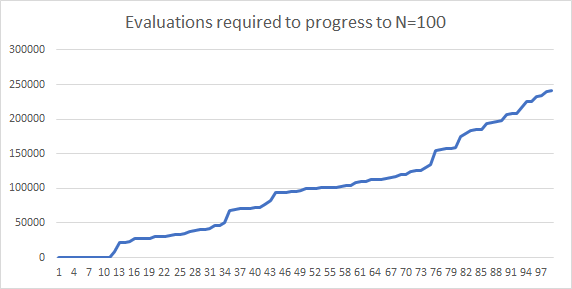
\includegraphics[width=10cm, height=5cm]{EvaluationProgress}
	\caption{Development of the number of evaluations required to obtain a solution for N = 100.}
\end{figure}


\section{Conclusions}
This research has shown that 

\begin{thebibliography}{99.}

\bibitem {Complexity} Gent I.P., Jefferson C., Nightingale P. 	Complexity of n-Queens Completion Journal of Artificial Intelligence Research 59 (2017) 

\bibitem {Pauls} E. Pauls, Das Maximalproblem der Damen auf dem Schachbrete, Deutsche Schachzeitung. Organ fur das Gesammte Schachleben 29 (5) (1874) 129–134.

\bibitem {Crawford} Kelly D. Crawford, Solving n-Queen problem using genetic algorithms SAC '92 Proceedings of the 1992 ACM/SIGAPP symposium on Applied computing,pp:1039-1047,1994 

\bibitem {Demes} Nowostawski, Mariusz and Poli, Riccardo. (1999). Dynamic Demes Parallel Genetic Algorithm. 10.1109/KES.1999.820128. 

\bibitem{27Queens} https://github.com/preusser/q27

\bibitem{AdvanceMutation} V. Jain, J.S. Prasad, (2018) Solving N-queen Problem Using Genetic Algorithm by Advance Mutation Operator. International Journal of Electrical and Computer Engineering

\bibitem{ACO} Khan, Salabat. Bilal, Mohsin. Sharif, Muhammad. Sajid Abbas. Malik, Baig, Abdul. (2010). Solution of n-Queen problem using ACO. 1 - 5. 10.1109/INMIC.2009.5383157. 

\bibitem{comparison} Martinjak, Ivica. Golub, M. (2007). Comparison of Heuristic Algorithms for the N-Queen Problem. 759 - 764. 10.1109/ITI.2007.4283867.

\bibitem{PSO}  Y. Wang, H. Lin, L. Yang (2012) "Swarm Refinement PSO for Solving N-Queens problem" Third International Conference on Bio-Inspired Computing and Applications. Kaoshiung 2012

\bibitem{Deadlock} M.M. Tanik, A graph model for deadlock prevention, Ph.D. Thesis, Texas A and M University, 1978

\bibitem{SIMD} M. M. Tanik, Parallel memory Allocation and Data Alignment in SIMD Machines, Parallel Algorithms and Applications, 1994

\bibitem{Circulant} M. M. Tanik, A Circulant Matrix Based Approach to Storage Schemes for Parallel Memory Systems,  in: Proceedings of the Fifth IEEE Symposium on Parallel and Distributed Processing

\bibitem{WSN} B. Stojkoska, D. Davcev, V. Trajkovik N-Queens based Algorithm for Moving Object Detection in Wireless Sensor Networks

\bibitem{Quantum} V> Torggler, P. Aumann, H. Ritsch, W. Lechner A Quantum N-Queens Solver (2018) 	arXiv:1803.00735 


\end{thebibliography}


\end{document}

